\documentclass[10pt]{article}

% ---------- Packages ----------
\usepackage[margin=0.7in]{geometry}
\usepackage{amsmath, amssymb, amsthm}
\usepackage{graphicx}
\usepackage{hyperref}
\usepackage{cleveref}
\usepackage{bm}
\usepackage{tikz}

% ---------- Reduce vertical space around display equations ----------
\setlength{\abovedisplayskip}{2pt}
\setlength{\belowdisplayskip}{2pt}
\setlength{\abovedisplayshortskip}{2pt}
\setlength{\belowdisplayshortskip}{2pt}
\setlength{\jot}{2pt}

% ---------- Tighter float spacing ----------
\setlength{\floatsep}{6pt plus 2pt minus 2pt}
\setlength{\textfloatsep}{8pt plus 2pt minus 2pt}
\setlength{\intextsep}{6pt plus 2pt minus 2pt}
\setlength{\abovecaptionskip}{4pt}
\setlength{\belowcaptionskip}{0pt}

% ---------- Tighten spacing in cases/array blocks ----------
\renewcommand{\arraystretch}{0.8}

% ---------- Theorem environments ----------
\newtheorem{theorem}{Theorem}[section]
\newtheorem{lemma}[theorem]{Lemma}
\newtheorem{proposition}[theorem]{Proposition}
\newtheorem{corollary}[theorem]{Corollary}
\theoremstyle{definition}
\newtheorem{definition}[theorem]{Definition}
\newtheorem{example}[theorem]{Example}
\theoremstyle{remark}
\newtheorem{remark}[theorem]{Remark}

% ---------- Title ----------
\title{Shocks, Weak Solutions, and Entropy: \\ An Exposition of Burgers' Equation}
\author{Russell Ng (A0213913M) \\ MA4221 Partial Differential Equations}
\date{\today}

\begin{document}

\maketitle

% ---------- Core exposition ----------
% =====================================================================
%  Sections 1--3: Introduction, Method of Characteristics, Breakdown of
%  classical solutions.
% =====================================================================

\section{Introduction}
\label{sec:motivation}

The viscous Burgers' equation
\begin{equation}
  \label{eq:viscous-burgers}
  u_t + u\,u_x = \nu\,u_{xx}, \qquad \nu>0,
\end{equation}
was introduced by Burgers \cite{burgers1948} as a one-dimensional model of
turbulence; it had appeared earlier in work of Bateman \cite{bateman1915}. It
has the form of the Navier--Stokes momentum equation without the pressure term,
and combines nonlinear advection with viscous diffusion. Setting $\nu=0$ gives
the inviscid equation
\begin{equation}
  \label{eq:inviscid-burgers}
  u_t + u\,u_x = 0,
\end{equation}
the scalar conservation law $u_t+f(u)_x=0$ with flux $f(u)=u^2/2$. Conservation
laws of this type arise in gas dynamics \cite{evans2010,leveque2002} and traffic flow \cite{lighthill1955}.
Burgers' equation is the simplest model in which nonlinearity alone produces
discontinuities: it is the standard test case for shock-capturing numerical
methods, and it is one of the few nonlinear equations that can be solved exactly,
through the Cole--Hopf transformation, so that every claim about shocks and entropy
can be checked against an explicit formula.

Classical solutions of \eqref{eq:inviscid-burgers} can break down in finite time
for smooth data (as soon as $u_0'$ is negative somewhere; see
Section~\ref{sec:shock-formation}), beyond which they can be continued only in
the weak sense, and weak solutions are not unique. Since
\eqref{eq:inviscid-burgers} idealises \eqref{eq:viscous-burgers} for small $\nu$,
with a shock appearing as a layer of thickness $O(\nu)$, the admissible weak
solutions should be those that arise as limits of viscous solutions. We
therefore ask \emph{why the inviscid Burgers' equation requires an entropy
condition, and why that condition is the correct one}. The answer is that the
entropy condition is the criterion selected by vanishing viscosity, a result due
to Hopf (Section~\ref{sec:extensions}). Sections~\ref{sec:characteristics} and
\ref{sec:shock-formation} locate the breakdown of classical solutions, and
Sections~\ref{sec:weak-solutions}--\ref{sec:riemann-problem} develop weak
solutions, their non-uniqueness and the entropy conditions that restore
uniqueness, culminating in the Riemann problem; Section~\ref{sec:extensions}
connects these with the Cole--Hopf formula, vanishing viscosity and Godunov's
method. The theory follows \cite[\S3.4]{evans2010}.

% =====================================================================

\section{Method of Characteristics}
\label{sec:characteristics}

Consider the initial value problem
\begin{equation}
  \label{eq:ivp}
  \begin{cases}
    u_t + u\, u_x = 0, & x \in \mathbb{R},\ t > 0, \\
    u(x,0) = u_0(x), & x \in \mathbb{R},
  \end{cases}
\end{equation}
with $u_0 \in C^1(\mathbb{R})$ in Sections~\ref{sec:characteristics} and
\ref{sec:shock-formation}. For discontinuous data, such as the Riemann data
\eqref{eq:riemann-data}, \eqref{eq:ivp} is understood in the weak sense of
Definition~\ref{def:weak-solution}.

\subsection{Characteristics}
\label{subsec:char-lines}

A \emph{characteristic} of a $C^1$ solution $u$ is a curve $x(t)$ satisfying
\begin{equation}
  \label{eq:char-ode-x}
  \dot{x}(t) = u(x(t), t).
\end{equation}
Along it,
\begin{equation}
  \label{eq:char-ode-u}
  \frac{d}{dt}\, u(x(t), t) = u_x\,\dot{x} + u_t = u_t + u\,u_x = 0 .
\end{equation}

Consequently $u$ is constant along each characteristic, so $\dot x$ is constant:
if $u$ is a $C^1$ solution of \eqref{eq:ivp} on $\mathbb{R}\times[0,T)$ and $x(t)$
solves \eqref{eq:char-ode-x} with $x(0)=x_0$, then for $0\le t<T$
\begin{equation}
  \label{eq:char-formula}
  u(x(t), t) = u_0(x_0), \qquad x(t) = x_0 + u_0(x_0)\, t,
\end{equation}
that is, characteristics are straight lines.

\subsection{The implicit solution formula}
\label{subsec:char-implicit-formula}

\begin{theorem}[Implicit solution via characteristics]
\label{thm:implicit-solution}
Let $u_0 \in C^1(\mathbb{R})$, $\Phi_t(x_0) = x_0 + u_0(x_0)\, t$, and
$T\in(0,\infty]$ such that for every $t\in[0,T)$, $\Phi_t'>0$ on $\mathbb{R}$
and $\Phi_t$ maps $\mathbb{R}$ onto $\mathbb{R}$. Then the function $u$ defined
implicitly by
\begin{equation}
  \label{eq:implicit-solution}
  u(x,t) = u_0(x_0), \qquad \text{where } x = x_0 + u_0(x_0)\, t,
\end{equation}
is the unique $C^1$ solution of \eqref{eq:ivp} on $\mathbb{R}\times[0,T)$.
\end{theorem}

\begin{proof}
\emph{Well-definedness and regularity.} Since $\Phi_t'>0$, $\Phi_t$ is
strictly increasing, hence bijective by hypothesis, so $u(x,t) =
u_0(\Phi_t^{-1}(x))$ is well defined. The function
$F(x_0,x,t)=x_0+u_0(x_0)t-x$ is $C^1$ with $\partial_{x_0}F=\Phi_t'>0$, so by
the implicit function theorem $x_0(x,t)=\Phi_t^{-1}(x)$ is $C^1$ in $(x,t)$
jointly (it is locally the unique root, and by injectivity coincides with the
global one). Hence $u=u_0(x_0(x,t))$ is $C^1$.

\emph{The PDE holds.} Write $x_0 = x_0(x,t) = \Phi_t^{-1}(x)$.
Differentiating $x = x_0 + u_0(x_0)\, t$ in $x$ and in $t$ gives
\begin{equation}
  \frac{\partial x_0}{\partial x} = \frac{1}{1 + u_0'(x_0)\,t},
  \qquad
  \frac{\partial x_0}{\partial t} = \frac{-u_0(x_0)}{1 + u_0'(x_0)\, t},
\end{equation}
both well defined since $\Phi_t'(x_0) = 1+u_0'(x_0)t > 0$. By the chain
rule applied to $u(x,t) = u_0(x_0(x,t))$,
\begin{equation}
  u_x = \frac{u_0'(x_0)}{1 + u_0'(x_0)\,t},
  \qquad
  u_t = \frac{-u_0(x_0)\, u_0'(x_0)}{1 + u_0'(x_0)\, t},
\end{equation}
so $u_t + u\,u_x = 0$, and $u(x,0)=u_0(x)$ since $\Phi_0=\mathrm{id}$.

\emph{Uniqueness.} Let $v$ be any $C^1$ solution of \eqref{eq:ivp} on
$\mathbb{R}\times[0,T)$, and fix $t\in(0,T)$, $x\in\mathbb{R}$. Solve backwards in time
the ODE $\dot\gamma(s)=v(\gamma(s),s)$, $\gamma(t)=x$ (the right-hand side is $C^1$,
hence locally Lipschitz, so there is a unique maximal solution). By
\eqref{eq:char-ode-u}, $v$ is constant along $\gamma$, hence so is $\dot\gamma$:
$\gamma$ is a straight line with bounded slope $v(x,t)$. It therefore stays
bounded and cannot blow up, so it extends back to $s=0$. Setting
$x_0=\gamma(0)$ we get $v(x,t)=v(x_0,0)=u_0(x_0)$ and $x=x_0+u_0(x_0)t$.
Thus every point $(x,t)$ lies on a characteristic coming from $t=0$, with
$x_0=\Phi_t^{-1}(x)$, and $v(x,t)=u_0(\Phi_t^{-1}(x))=u(x,t)$.
\end{proof}

\begin{corollary}[Local existence]
\label{cor:local-existence}
Let $u_0 \in C^1(\mathbb{R})$ with $m := \inf_{x_0} u_0'(x_0) > -\infty$,
and set $T=\infty$ if $m\ge0$ and $T=-1/m$ if $m<0$. Then
\eqref{eq:ivp} has a unique $C^1$ solution on $\mathbb{R}\times[0,T)$,
given by \eqref{eq:implicit-solution}.
\end{corollary}

\begin{proof}
Fix $t\in[0,T)$ and put $\kappa_t := 1+\min(m,0)\,t$, so $\kappa_t>0$ and
$\Phi_t'(x_0)=1+u_0'(x_0)t\ge \kappa_t$ for every $x_0$. Two consequences
follow. (i) $\Phi_t$ is strictly increasing, hence injective. (ii) By the
mean value theorem $\Phi_t(x_0)-\Phi_t(0)\ge \kappa_t x_0$ for $x_0\ge0$ and
$\le \kappa_t x_0$ for $x_0\le0$, so $\Phi_t(x_0)\to\pm\infty$ as
$x_0\to\pm\infty$; by continuity $\Phi_t$ is onto $\mathbb{R}$.
Hence the hypotheses of Theorem~\ref{thm:implicit-solution} hold on
$[0,T)$.
\end{proof}

\begin{remark}
\label{rem:hypothesis-u0prime}
The uniform lower bound $\Phi_t'\ge \kappa_t>0$, not strict monotonicity alone,
gives surjectivity: for $u_0(x)=(\arctan x-x)/t_0$ one has $\Phi_{t_0}(x)=\arctan x$,
strictly increasing with $\Phi_{t_0}'>0$ but not onto $\mathbb{R}$. The
hypothesis $m>-\infty$ cannot be dropped either: for $u_0(x)=x^2$,
$\Phi_t(x)=x+tx^2$ is not injective for any $t>0$, since $\Phi_t'(x)<0$ for
$x<-1/(2t)$.
\end{remark}

% =====================================================================

\section{Breakdown of Classical Solutions}
\label{sec:shock-formation}

\subsection{Blow-up of the derivative and the envelope}
\label{subsec:shock-derivative-blowup}

By the proof of Theorem~\ref{thm:implicit-solution},
\begin{equation}
  \label{eq:ux-formula}
  u_x(x,t) = \frac{u_0'(x_0)}{1 + u_0'(x_0)\, t}, \qquad x = x_0 + u_0(x_0)\, t.
\end{equation}
The formula holds as long as the classical solution exists
(Corollary~\ref{cor:local-existence}, that is, for $t<-1/\inf u_0'$). If
$u_0'(x_0) \geq 0$ the denominator is at least $1$, and $u_x$ remains bounded
along that characteristic. If $u_0'(x_0) < 0$, the right-hand side, regarded as
a formal expression along the characteristic through $x_0$, has a vanishing
denominator at $t = -1/u_0'(x_0)$; the classical solution itself ceases to exist
no later than this time, and strictly earlier unless $x_0$ minimises $u_0'$
(Proposition~\ref{prop:shock-time}). The characteristics
\begin{equation}
  \label{eq:char-family}
  x(x_0, t) = x_0 + u_0(x_0)\, t, \qquad x_0 \in \mathbb{R},
\end{equation}
have an envelope where $\partial x/\partial x_0 = 1 + u_0'(x_0)\,t = 0$, that
is, where $\Phi_t'(x_0)=0$; this concerns the family \eqref{eq:char-family},
not the solution beyond its first breakdown.

\subsection{The breakdown time}
\label{subsec:shock-time}

\begin{proposition}[Breakdown time]
\label{prop:shock-time}
Let $u_0 \in C^1(\mathbb{R})$ with $m := \inf_{x_0} u_0'(x_0)\in(-\infty,0)$, and
set
\begin{equation}
  \label{eq:shock-time}
  T^* = \frac{-1}{m}.
\end{equation}
Then a $C^1$ solution exists on $\mathbb{R} \times [0,T^*)$, with
$\sup_x|u_x(\cdot,t)|\to\infty$ as $t\uparrow T^*$, and for every $T>T^*$ no
$C^1$ solution exists on $\mathbb{R}\times[0,T)$. If the infimum is attained at
$x_0=a$, the solution degenerates at time $T^*$ at the points
\begin{equation}
  \label{eq:shock-location}
  x^* = a + u_0(a)\, T^*, \qquad t^* = T^*.
\end{equation}
\end{proposition}

\begin{proof}
Since $r \mapsto -1/r$ is strictly increasing on $(-\infty,0)$ and
$u_0'(x_0) \geq m$ everywhere, $-1/u_0'(x_0) \geq T^*$ whenever $u_0'(x_0)<0$, so
$\Phi_t'>0$ throughout $[0,T^*)$ and Corollary~\ref{cor:local-existence} gives a
classical solution $u$ there. Choosing $x_n$ with $u_0'(x_n)\to m$,
\eqref{eq:ux-formula} gives $u_x\to m/(1+mt)$ at the point with foot $x_n$, so
$\sup_x|u_x(\cdot,t)|\ge|m|/(1-|m|t)\to\infty$ as $t\uparrow T^*$.

Now let $T>T^*$ and suppose $v$ is a $C^1$ solution on $\mathbb{R}\times[0,T)$.
Since $m<-1/T$, there is $a$ with $u_0'(a)<-1/T$, that is,
$\tau:=-1/u_0'(a)<T$. By \eqref{eq:char-formula} (the characteristic
through $(a',0)$ has bounded slope, hence exists on all of $[0,T)$),
$v(a'+tu_0(a'),t)=u_0(a')$ for every $a'$ and $t<T$. Differentiating in $a'$ at
$a'=a$ gives
\begin{equation*}
  v_x\big(a+tu_0(a),t\big)\,\big(1+t\,u_0'(a)\big)=u_0'(a),
\end{equation*}
and at $t=\tau$ the left side vanishes while the right side is negative, a
contradiction. Finally, if the infimum is attained at $a$, then along the
characteristic from $a$ we have $u_x=m/(1+mt)\to-\infty$ as $t\uparrow T^*$, at
points tending to $(x^*,T^*)$ by \eqref{eq:char-family}.
\end{proof}

\begin{remark}
\label{rem:singularity-vs-shock}
Assume that $u_0$ is bounded, that the infimum $m$ of $u_0'$ is attained, and
that $\{u_0'=m\}$ contains no interval. Then $\Phi_{T^*}'\ge0$ vanishes only on a
set with empty interior, so $\Phi_{T^*}$ is strictly increasing; it is onto
$\mathbb{R}$ because $u_0$ is bounded, so $\Phi_{T^*}(x_0)\to\pm\infty$ as
$x_0\to\pm\infty$ (this replaces the argument of
Corollary~\ref{cor:local-existence}, which degenerates at $t=T^*$). Thus exactly
one characteristic reaches each point at time $T^*$, and $u$, bounded by
$\sup|u_0|$ by \eqref{eq:char-formula}, develops at $(x^*,T^*)$ only a gradient
catastrophe, $|u_x|\to\infty$. If instead $u_0'\equiv m$ on an interval, then
$\Phi_{T^*}$ is constant on it and characteristics carrying different values of
$u_0$ meet at one point at time $T^*$, so one expects a discontinuity to form
at $T^*$; this is not proved here (it follows from the Lax--Oleinik formula,
Remark~\ref{rem:lax-oleinik}).
\end{remark}

\subsection{Example: $u_0=-\arctan x$}
\label{subsec:arctan-breakdown}

Here $u_0'(x_0)=-1/(1+x_0^2)\in[-1,0)$ is minimised at $a=0$ with $m=-1$, so
Proposition~\ref{prop:shock-time} gives $T^*=1$ and $x^*=0$: the singularity
first appears at $(x^*,t^*)=(0,1)$ (Figure~\ref{fig:characteristics}). Here
$\Phi_t'(x_0)=1-t/(1+x_0^2)$ first vanishes at $t=1$, at $x_0=0$. At $t=1$ the
map $\Phi_1(x_0)=x_0-\arctan x_0$ is strictly increasing but its inverse is
not $C^1$ at $0$; for $t>1$, $\Phi_t'<0$ on an interval around $x_0=0$, so
$\Phi_t$ is not injective and characteristics cross.
Geometrically, the characteristic from $x_0$ has speed $u_0(x_0)=-\arctan x_0$, so
those starting near $0$, where $u_0$ falls fastest, converge on one another first,
and the crossing begins at the single point $(0,1)$ rather than everywhere at once.
After that time $u$ would take several values at a point, which is why a notion of
solution that allows jumps is needed.

\begin{figure}[htbp]
\centering
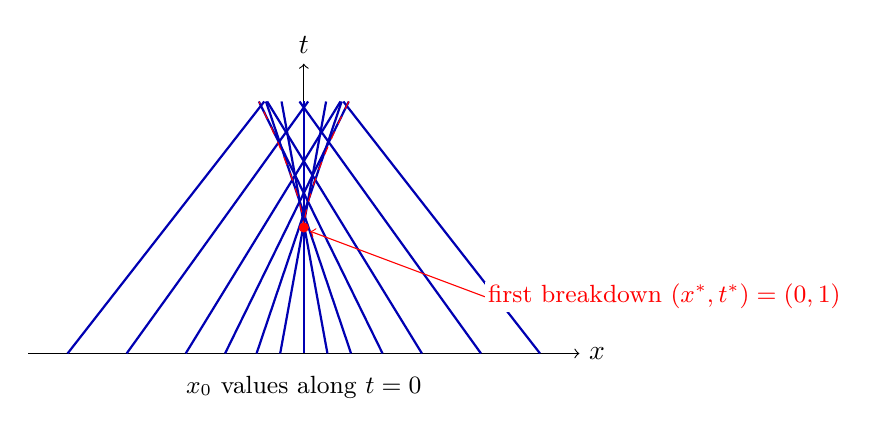
\begin{tikzpicture}[x=1cm,y=1.6cm]
  \draw[->] (-3.5,0) -- (3.5,0) node[right] {$x$};
  \draw[->] (0,0) -- (0,2.3) node[above] {$t$};
  % characteristics x = x0 - arctan(x0) t, drawn for 0 <= t <= 2
  \foreach \xz in {-3,-2.25,-1.5,-1,-0.6,-0.3,0,0.3,0.6,1,1.5,2.25,3}{
    \pgfmathsetmacro{\xe}{\xz - rad(atan(\xz))*2}
    \draw[thick, blue!70!black] (\xz,0) -- (\xe,2);
  }
  % envelope: t = 1+s^2, x = s - arctan(s)(1+s^2)
  \draw[red, dashed, domain=-1:1, samples=40, smooth, variable=\s]
    plot ({\s - rad(atan(\s))*(1+\s*\s)}, {1+\s*\s});
  \filldraw[red] (0,1) circle (1.6pt);
  \draw[red, ->] (2.3,0.45) -- (0.08,0.97);
  \node[red, right, fill=white, inner sep=1pt] at (2.3,0.45) {\small first breakdown $(x^*,t^*)=(0,1)$};
  \node[below] at (0,-0.1) {\small $x_0$ values along $t=0$};
\end{tikzpicture}
\caption{Characteristics $x=x_0-\arctan(x_0)\,t$ for $u_0=-\arctan x$, with
their envelope (red, dashed), which has a cusp at the first breakdown
$(x^*,t^*)=(0,1)$. Inside the cusp ($t>1$) three characteristics pass through
each point.}
\label{fig:characteristics}
\end{figure}

By Remark~\ref{rem:lax-oleinik} and Theorem~\ref{thm:oleinik-uniqueness}, the
entropy solution is given by the Lax--Oleinik formula \eqref{eq:lax-oleinik}.
Here $V(y)=-\big(y\arctan y-\tfrac12\ln(1+y^2)\big)$ is even, and
\begin{equation*}
  \partial_yG(x,y,t)=\frac{\Phi_t(y)-x}{t},\qquad
  \partial_y^2G=\frac{\Phi_t'(y)}{t}=\frac1t-\frac1{1+y^2},\qquad
  \Phi_t(y)=y-t\arctan y .
\end{equation*}

\emph{$t\le1$.} Then $\partial_y^2G>0$ except possibly at $y=0$, so $G(x,\cdot,t)$ is strictly convex and its unique
minimiser is the unique critical point, the characteristic foot $\Phi_t^{-1}(x)$.
Thus the entropy solution is the classical solution
\eqref{eq:implicit-solution}.

\emph{$t>1$.} Now $\Phi_t$ is odd, with $\Phi_t'<0$ exactly on $(-s,s)$,
$s=\sqrt{t-1}$. Fix $x>0$. Since $G(x,y,t)-G(x,-y,t)=-2xy/t$, no minimiser has
$y<0$, and $y=0$ is not one, since $\partial_yG(x,0,t)=-x/t<0$. On $(0,s]$ we
have $\Phi_t\le0<x$, and on $(s,\infty)$ $\Phi_t$ increases from a negative value
to $+\infty$. Hence $G(x,\cdot,t)$ has exactly one critical point
$y_+(x,t)>s$ in $(0,\infty)$, with $\Phi_t'(y_+)>0$; it is the unique
minimiser, and $u=(x-y_+)/t=-\arctan y_+$ is smooth in $x$ by the implicit
function theorem; by oddness the same holds for $x<0$. At $x=0$ the function
$G(0,\cdot,t)$ is even with $\partial_y^2G(0,0,t)=(1-t)/t<0$, so $0$ is not a
minimiser, and the minimisers are $\pm y^*$, where $y^*>0$ is the unique
positive root of $y^*=t\arctan y^*$(the minimum is attained at two symmetric points). Therefore, for $t>1$, the entropy
solution is smooth off $x=0$ and has exactly one jump, stationary at $x=0$ with
\begin{equation*}
  u_\ell=-u_r=\frac{y^*}{t}=\arctan y^*\in(0,\tfrac\pi2).
\end{equation*}
Moreover $y^*=\sqrt{3(1-1/t)}\,(1+o(1))$ as $t\downarrow1$ from
$\arctan y=y-y^3/3+O(y^5)$, so $u_\ell\sim\sqrt{3(t-1)}$, and $y^*>s\to\infty$
gives $u_\ell\to\pi/2$ as $t\to\infty$, matching the limits $u_0(\mp\infty)=\pm\pi/2$.     % Sections 1--3: motivation, characteristics, breakdown
% =====================================================================
%  Sections 4--7: Weak solutions, Non-uniqueness, Entropy condition,
%  Riemann problem.
% =====================================================================

\section{Weak Solutions}
\label{sec:weak-solutions}

From here on we assume $u_0\in L^\infty(\mathbb{R})$, whereas Sections~\ref{sec:characteristics}--\ref{sec:shock-formation}
allowed unbounded $C^1$ data; weak solutions are bounded by
Definition~\ref{def:weak-solution}, so they do not continue every classical
solution considered there.

\subsection{The integral formulation}
\label{subsec:integral-form}

Let $f(u)=u^2/2$. If $u$ is a $C^1$ solution of $u_t + f(u)_x = 0$ with
$u(\cdot,0)=u_0$ and $\varphi \in C_c^1(\mathbb{R} \times [0,\infty))$, then
integration by parts in $x$ and $t$ gives
\begin{equation}
  \label{eq:weak-derivation}
  0 = \int_0^\infty\!\!\int_{\mathbb{R}} \big(u_t + f(u)_x\big)\varphi\, dx\, dt
  = -\int_0^\infty\!\!\int_{\mathbb{R}} \big(u\,\varphi_t + f(u)\,\varphi_x\big)\, dx\, dt
  - \int_{\mathbb{R}} u_0(x)\, \varphi(x,0)\, dx .
\end{equation}
Since the right-hand side requires no differentiability of $u$, it can be used to define solutions of lower regularity.

\begin{definition}[Weak solution]
\label{def:weak-solution}
Let $u_0\in L^\infty(\mathbb{R})$. A function $u \in
L^\infty(\mathbb{R}\times(0,\infty))$ is a \emph{weak solution} of
\eqref{eq:ivp} (with data $u_0$) if
\begin{equation}
  \label{eq:weak-formulation}
  \int_0^\infty\!\!\int_{\mathbb{R}} \big(u\,\varphi_t + f(u)\,\varphi_x\big)\, dx\, dt
  + \int_{\mathbb{R}} u_0(x)\, \varphi(x,0)\, dx = 0
\end{equation}
for every $\varphi \in C_c^1(\mathbb{R}\times[0,\infty))$.
\end{definition}

Reversing the integration by parts in \eqref{eq:weak-derivation} and applying
the fundamental lemma of the calculus of variations shows that a bounded
$u\in C^1(\mathbb{R}\times[0,\infty))$ is a weak solution with data $u_0$ if and
only if it is a classical solution with $u(\cdot,0)=u_0$.

\subsection{Piecewise smooth functions and the Rankine--Hugoniot condition}
\label{subsec:rankine-hugoniot}

\begin{definition}[Piecewise $C^1$ function]
\label{def:piecewise}
Let $\sigma_1,\dots,\sigma_k:[0,\infty)\to\mathbb{R}$ be $C^1$ with $\sigma_1(t)<\dots<
\sigma_k(t)$ for $t>0$ (the curves may start at a common point when $t=0$).
Put $\sigma_0\equiv-\infty$, $\sigma_{k+1}\equiv+\infty$ and
$\Omega_i=\{(x,t):\ t>0,\ \sigma_i(t)<x<\sigma_{i+1}(t)\}$ for $i=0,\dots,k$. A
bounded function $u$ is \emph{piecewise $C^1$ with respect to
$\sigma_1,\dots,\sigma_k$} if on each $\Omega_i$ it is $C^1$ and $u,u_x,u_t$ extend
continuously to the closure of $\Omega_i$ in $\mathbb{R}\times(0,\infty)$, that is, to the points of the boundary curves with $t>0$. Along $x=\sigma_i(t)$ we
write $u_\ell(t)$ and $u_r(t)$ for the limits taken from $\Omega_{i-1}$
and $\Omega_i$ respectively.
\end{definition}

The restriction to finitely many $C^1$ curves is made so that checking the weak
formulation reduces to the PDE on each region together with the Rankine--Hugoniot
condition on each curve (Lemma~\ref{lem:boundary-identity}). This suffices to verify the
explicit solutions of Sections~\ref{sec:nonuniqueness}--\ref{sec:riemann-problem},
but it is not a general description of entropy solutions: it excludes, for instance, a gradient
catastrophe at an interior time such as $(0,1)$ in Section~\ref{subsec:arctan-breakdown}, and
interacting shocks. General solutions are covered by
Definition~\ref{def:weak-solution} and the existence theory cited in
Section~\ref{sec:entropy-condition}.

\begin{lemma}[Boundary identity]
\label{lem:boundary-identity}
Let $u$ be piecewise $C^1$ with respect to $\sigma_1,\dots,\sigma_k$ and satisfy
$u_t+f(u)_x=0$ classically in each $\Omega_i$. Then for every
$\varphi\in C_c^1(\mathbb{R}\times[0,\infty))$ and every $\varepsilon>0$,
\begin{equation}
  \label{eq:boundary-identity}
  \iint_{t>\varepsilon}\big(u\varphi_t+f(u)\varphi_x\big)\,dx\,dt
  = -\int_{\mathbb{R}} u(x,\varepsilon)\,\varphi(x,\varepsilon)\,dx
  +\sum_{i=1}^k\int_\varepsilon^\infty\Big[\big(f(u_\ell)-\sigma_i'u_\ell\big)
    -\big(f(u_r)-\sigma_i'u_r\big)\Big]\varphi(\sigma_i(t),t)\,dt .
\end{equation}
\end{lemma}

\begin{proof}
On each $\Omega_i^\varepsilon=\Omega_i\cap\{t>\varepsilon\}$ (a Lipschitz
domain, bounded after intersecting with $\operatorname{supp}\varphi$) the
vector field $\varphi\,(f(u),u)$ (components in the $(x,t)$ order) is $C^1$ up
to the boundary, and its divergence is $u\varphi_t+f(u)\varphi_x$ because
$u_t+f(u)_x=0$ there. The divergence theorem gives
\begin{equation*}
  \iint_{\Omega_i^\varepsilon}(u\varphi_t+f(u)\varphi_x)\,dx\,dt
  = \oint \varphi\,\big(f(u)\,n_x+u\,n_t\big)\,d\sigma ,
\end{equation*}
where $d\sigma\,\mathbf n$ equals $(1,-\sigma_{i+1}')\,dt$ on the right edge
$x=\sigma_{i+1}(t)$, $(-1,\sigma_i')\,dt$ on the left edge $x=\sigma_i(t)$, and
$(0,-1)\,dx$ on the bottom edge $t=\varepsilon$. Summing over $i$, the bottom
edges give $-\int u(x,\varepsilon)\varphi(x,\varepsilon)\,dx$, and the two
sides of each curve $x=\sigma_i(t)$ (from $\Omega_{i-1}$ on its left, $\Omega_i$ on
its right) combine into the bracket in \eqref{eq:boundary-identity}.
\end{proof}

\begin{theorem}[Rankine--Hugoniot condition]
\label{thm:rankine-hugoniot}
Let $u$ be piecewise $C^1$ with respect to $\sigma_1,\dots,\sigma_k$, and a weak
solution of \eqref{eq:ivp} for some data $u_0\in L^\infty$. Then $u_t+f(u)_x=0$
classically in each $\Omega_i$, and along each curve $x=\sigma_i(t)$, $t>0$,
\begin{equation}
  \label{eq:rh-jump}
  f(u_\ell(t)) - f(u_r(t)) = \sigma_i'(t)\,\big(u_\ell(t)-u_r(t)\big).
\end{equation}
In particular, wherever $u_\ell(t)\neq u_r(t)$, and for $f(u)=u^2/2$,
\begin{equation}
  \label{eq:rankine-hugoniot-burgers}
  \sigma_i'(t) = \frac{f(u_\ell) - f(u_r)}{u_\ell - u_r} = \frac{u_\ell(t) + u_r(t)}{2}.
\end{equation}
\end{theorem}

\begin{proof}
Test functions $\varphi$ supported in a single $\Omega_i$ give
$\iint (u\varphi_t+f(u)\varphi_x)=0$, so $u_t+f(u)_x=0$ in the weak sense
there; as $u$ is $C^1$ on $\Omega_i$, this holds classically, so
Lemma~\ref{lem:boundary-identity} applies.

Now fix $t_0>0$, an index $i$, and $\varphi\in C_c^1(\mathbb{R}\times
(0,\infty))$ supported in a small ball around $(\sigma_i(t_0),t_0)$ meeting no
other curve. Take $\varepsilon$ below the support of $\varphi$ in
\eqref{eq:boundary-identity}: the left side is $0$ by
\eqref{eq:weak-formulation} (as $\varphi(\cdot,0)=0$), the bottom term
vanishes, and only the curve $x=\sigma_i(t)$ contributes to the sum, so
\begin{equation*}
  0=\int_0^\infty\Big[\big(f(u_\ell)-\sigma_i'u_\ell\big)
    -\big(f(u_r)-\sigma_i'u_r\big)\Big]\varphi(\sigma_i(t),t)\,dt .
\end{equation*}
Since $\varphi(\sigma_i(t),t)$ may be any $C^1$ function of $t$ with small
support, the bracket vanishes identically, which is \eqref{eq:rh-jump}.
The first form of \eqref{eq:rankine-hugoniot-burgers} follows by division, and
the second from $f(u_\ell)-f(u_r)=\tfrac12(u_\ell-u_r)(u_\ell+u_r)$.
\end{proof}

\begin{proposition}[Piecewise smooth weak solutions]
\label{prop:piecewise-weak}
Let $u_0\in L^\infty(\mathbb{R})$ and let $u$ be piecewise $C^1$ with
respect to $\sigma_1,\dots,\sigma_k$. Suppose
\begin{enumerate}
  \item[\textup{(i)}] $u_t+f(u)_x=0$ classically in each $\Omega_i$;
  \item[\textup{(ii)}] the jump relation \eqref{eq:rh-jump} holds along
    each curve $x=\sigma_i(t)$, $t>0$ (automatic where $u$ is continuous
    across the curve);
  \item[\textup{(iii)}] $u(x,t)\to u_0(x)$ as
    $t\to0^+$ for every $x\notin\{\sigma_1(0),\dots,\sigma_k(0)\}$.
\end{enumerate}
Then $u$ is a weak solution of \eqref{eq:ivp} with data $u_0$.
\end{proposition}

\begin{proof}
Fix $\varphi\in C_c^1(\mathbb{R}\times[0,\infty))$ and $\varepsilon>0$. By (i),
Lemma~\ref{lem:boundary-identity} applies, and by (ii) every term of the sum in
\eqref{eq:boundary-identity} vanishes, so
\begin{equation*}
  \iint_{t>\varepsilon}\big(u\varphi_t+f(u)\varphi_x\big)\,dx\,dt
  = -\int_{\mathbb{R}} u(x,\varepsilon)\,\varphi(x,\varepsilon)\,dx .
\end{equation*}
Let $\varepsilon\to0^+$. The left side tends to the integral over
$t>0$ (bounded integrand, compact support). On the right,
$\varphi(\cdot,\varepsilon)\to\varphi(\cdot,0)$ uniformly and, by (iii),
$u(\cdot,\varepsilon)\to u_0$ almost everywhere with $|u|\le\|u\|_\infty$,
so dominated convergence gives $-\int u_0\varphi(\cdot,0)\,dx$. This is
\eqref{eq:weak-formulation}; since the argument is run on $t>\varepsilon$, the
curves are allowed to meet at $t=0$.
\end{proof}

% =====================================================================

\section{Non-Uniqueness of Weak Solutions}
\label{sec:nonuniqueness}

Consider \eqref{eq:ivp} with the Riemann data
\begin{equation}
  \label{eq:riemann-data}
  u_0(x) = \begin{cases} 0, & x < 0, \\ 1, & x > 0. \end{cases}
\end{equation}
Characteristics emanate from $x_0<0$ with speed $0$ and from $x_0>0$ with
speed $1$, so none covers the wedge $0<x<t$.

\begin{proposition}[Non-uniqueness]
\label{prop:nonuniqueness}
The functions
\begin{align}
  \label{eq:shock-solution}
  u_A(x,t) &= \begin{cases} 0, & x < t/2, \\ 1, & x > t/2, \end{cases}\\
  \label{eq:rarefaction-solution}
  u_B(x,t) &= \begin{cases}
    0, & x \le 0, \\
    x/t, & 0 < x < t, \\
    1, & x \ge t,
  \end{cases}
\end{align}
are distinct weak solutions of \eqref{eq:ivp} with data \eqref{eq:riemann-data};
they differ on the wedge $0<x<t$.
\end{proposition}

\begin{proof}
Both are covered by Proposition~\ref{prop:piecewise-weak}. For $u_A$ take $k=1$ and
$\sigma_1(t)=t/2$: $u_A$ is constant on each side and the jump moves at the
Rankine--Hugoniot speed $(0+1)/2=\tfrac12$ of \eqref{eq:rankine-hugoniot-burgers}.
For $u_B$ take $k=2$, $\sigma_1\equiv0$, $\sigma_2(t)=t$: $u_B$ is constant on the
outer regions, solves the PDE on $0<x<t$ since
$(u_B)_t+u_B(u_B)_x=-x/t^2+(x/t)(1/t)=0$, and is continuous across both curves,
so \eqref{eq:rh-jump} holds trivially. In both cases $u(\cdot,t)\to u_0$ at
every $x\ne0$.
\end{proof}

\begin{remark}[An infinite family]
\label{rem:infinite-family}
More generally, for $\alpha\in\mathbb{R}$ the function equal to $0$ for
$x<\tfrac\alpha2t$, to $\alpha$ for $\tfrac\alpha2t<x<\tfrac{1+\alpha}2t$ and to
$1$ for $x>\tfrac{1+\alpha}2t$ is a weak solution with data
\eqref{eq:riemann-data} by Proposition~\ref{prop:piecewise-weak} (its two jumps
move at their Rankine--Hugoniot speeds $\alpha/2<(1+\alpha)/2$); we denote it
$u^{(\alpha)}$, and $u^{(0)}=u^{(1)}=u_A$.\end{remark}

% =====================================================================

\section{The Entropy Condition}
\label{sec:entropy-condition}

\subsection{The Lax shock condition}
\label{subsec:lax-condition}

\begin{definition}[Lax shock condition]
\label{def:lax}
Let $u$ be a weak solution of a scalar conservation law $u_t+f(u)_x=0$
with $f\in C^2$, $f''>0$, and suppose $u$ has a jump discontinuity along a $C^1$
curve $x=\sigma(t)$ with left and right limits $u_\ell(t)$, $u_r(t)$. The jump
satisfies the \emph{Lax shock condition} if
\begin{equation}
  \label{eq:lax-condition}
  f'(u_\ell(t)) > \sigma'(t) > f'(u_r(t))
\end{equation}
for all $t$.
\end{definition}

For strictly convex $f$ the Rankine--Hugoniot speed $(f(u_\ell)-f(u_r))/(u_\ell-u_r)$
lies strictly between $f'(u_\ell)$ and $f'(u_r)$, in the order of $u_\ell,u_r$
(mean value theorem), so \eqref{eq:lax-condition} holds if and only if
$u_\ell>u_r$. For $f(u)=u^2/2$ and $\sigma'=(u_\ell+u_r)/2$, \eqref{eq:lax-condition} reduces to
\begin{equation}
  \label{eq:lax-burgers}
  u_\ell > \frac{u_\ell+u_r}{2} > u_r
  \quad \Longleftrightarrow \quad
  u_\ell > u_r.
\end{equation}
Thus characteristics on both sides run into the shock. The Lax condition is local:
it tests one jump at a time and says nothing about the smooth parts of the solution,
whereas the Oleinik condition of the next subsection is global in $x$ and does
(Remark~\ref{rem:lax-vs-oleinik}). It also depends on convexity: for non-convex
$f$ the Lax inequalities no longer characterise admissible shocks, and one passes to
Oleinik's condition~E or to Kru\v{z}kov's entropy inequalities
\cite{kruzhkov1970,leveque2002}, which we do not pursue. Since the Lax condition
constrains jumps only, its derivation from viscosity, giving $u_\ell>u_r$, is
deferred to Proposition~\ref{prop:viscous-profile}.

\subsection{Entropy solutions: the Oleinik condition}
\label{subsec:oleinik}

\begin{definition}[Entropy solution]
\label{def:entropy-solution}
A weak solution $u\in L^\infty$ of \eqref{eq:ivp} is an \emph{entropy
solution} if
\begin{equation}
  \label{eq:oleinik}
  u(x+z,t)-u(x,t)\ \le\ \frac{z}{t}
  \qquad\text{for every }z>0\text{ and a.e.\ }(x,t)\in\mathbb{R}\times(0,\infty).
\end{equation}
\end{definition}

The one-sided Lipschitz bound \eqref{eq:oleinik} is due to Oleinik
\cite{oleinik1957}. It prevents $u(\cdot,t)$ from increasing at a rate exceeding
$1/t$, which is what excludes upward jumps (Lemma~\ref{lem:oleinik-lax}).

\begin{remark}[Entropy inequalities]
\label{rem:entropy-inequality}
The name refers to the following mechanism. Let $\eta$ be convex with entropy
flux $q$, $q'=\eta'f'$. A smooth solution of \eqref{eq:viscous-burgers} satisfies
\begin{equation*}
  \eta(u)_t+q(u)_x=\nu\,\eta(u)_{xx}-\nu\,\eta''(u)\,u_x^2\ \le\ \nu\,\eta(u)_{xx},
\end{equation*}
so that, as $\nu\to0$, the limit satisfies $\eta(u)_t+q(u)_x\le0$ in the sense of
distributions: entropy is dissipated across shocks, never produced. For Burgers'
equation, requiring this for all convex $\eta$ is equivalent to
\eqref{eq:oleinik} \cite{kruzhkov1970,leveque2002}; we use \eqref{eq:oleinik}
because it is the form needed for uniqueness, and do not prove the equivalence.
\end{remark}

\begin{lemma}[Oleinik implies Lax]
\label{lem:oleinik-lax}
Let $u$ be a piecewise $C^1$ entropy solution of Burgers' equation. Then
every jump of $u$ satisfies the Lax condition \eqref{eq:lax-condition},
equivalently $u_\ell>u_r$.
\end{lemma}

\begin{proof}
Fix a curve $x=\sigma(t)$ and $t_0>0$ with $u_\ell(t_0)\ne u_r(t_0)$. For $z>0$ small
enough that $[\sigma(t_0)-z,\sigma(t_0)+z]$ meets no other curve, there is a
neighbourhood $N$ of $(\sigma(t_0),t_0)$ in which every pair $(x,t),(x+z,t)$ with
$x<\sigma(t)<x+z$ lies on opposite sides of the curve $x=\sigma(t)$ only, where
$u$ is $C^1$. Both sides of \eqref{eq:oleinik} are continuous on the open set
$\{(x,t)\in N: x<\sigma(t)<x+z\}$, so the a.e.\ inequality holds at every point of
it, in particular at $(\sigma(t_0)-z/2,t_0)$. Letting $z\to0$, the left side
tends to $u_r(t_0)-u_\ell(t_0)$ and the right side to $0$. Hence $u_r\le u_\ell$ at
$t_0$, and since the limits differ, $u_\ell>u_r$.
\end{proof}

\begin{remark}
\label{rem:lax-vs-oleinik}
For a piecewise $C^1$ solution with locally finitely many jumps,
\eqref{eq:oleinik} holds if and only if each jump satisfies $u_\ell>u_r$ and
$u_x\le 1/t$ on the smooth pieces. The Lax condition is thus a local admissibility
condition, pointwise on each jump, and is the local form of \eqref{eq:oleinik}
at jumps for piecewise $C^1$ solutions. The Oleinik bound is global in $x$: it
also constrains the smooth parts ($u_x\le1/t$), and it is meaningful for general
$L^\infty$ weak solutions, for which no jump structure is available. It is the
bound used in the uniqueness proof below. Lemma~\ref{lem:oleinik-lax} is used only
to test the explicit piecewise $C^1$ solutions; the uniqueness theorem
(Theorem~\ref{thm:oleinik-uniqueness}) assumes \eqref{eq:oleinik} directly and does
not pass through the Lax condition, so there is no circularity.
\end{remark}

\begin{proposition}
\label{prop:entropy-selects-B}
For the Riemann data \eqref{eq:riemann-data} ($u_\ell=0<u_r=1$), the
rarefaction solution $u_B$ of \eqref{eq:rarefaction-solution} is an
entropy solution, while the shock solution $u_A$ of
\eqref{eq:shock-solution} and every $u^{(\alpha)}$ of
Remark~\ref{rem:infinite-family} are not.
\end{proposition}

\begin{proof}
\emph{$u_B$ is entropy.} Write $u_B(x,t)=\min\{\max\{x/t,0\},1\}$, the
composition of $x\mapsto x/t$ with the $1$-Lipschitz function
$y\mapsto\min\{\max\{y,0\},1\}$. Hence $u_B(\cdot,t)$ is $(1/t)$-Lipschitz
and $u_B(x+z,t)-u_B(x,t)\le z/t$, which is \eqref{eq:oleinik}.

\emph{$u_A$ and $u^{(\alpha)}$ are not.} Each contains an upward jump ($0\to1$ for
$u_A$; $0\to\alpha$ if $\alpha>0$ and $\alpha\to1$ if $\alpha\le0$ for
$u^{(\alpha)}$), which Lemma~\ref{lem:oleinik-lax} excludes. (Directly, for $u_A$
and $z<t$ the increment equals $1>z/t$ for every $x\in(t/2-z,t/2)$.)
\end{proof}

\subsection{Uniqueness}
\label{subsec:entropy-uniqueness}

\begin{theorem}[{Oleinik; \cite[\S3.4.3]{evans2010}}]
\label{thm:oleinik-uniqueness}
For $u_0 \in L^\infty(\mathbb{R})$ and $f(u)=u^2/2$, the initial value
problem $u_t+f(u)_x=0$, $u(\cdot,0)=u_0$, has at most one entropy solution in
the sense of Definition~\ref{def:entropy-solution}, up to a set of measure
zero. An entropy solution exists: the Lax--Oleinik solution
\cite[\S3.4.2]{evans2010} is a weak solution satisfying
\eqref{eq:oleinik} (Remark~\ref{rem:lax-oleinik}).
\end{theorem}

(Evans proves uniqueness under the weaker bound
$u(x+z,t)-u(x,t)\le C(1+1/t)\,z$, valid for general uniformly convex fluxes,
which every solution of \eqref{eq:oleinik} satisfies with $C=1$.) The proof in \cite[\S3.4.3]{evans2010} proceeds by duality. The difference
$w=u_1-u_2$ of two entropy solutions with the same data satisfies
$\iint w\,(\varphi_t+b\,\varphi_x)\,dx\,dt=0$ for all test functions $\varphi$,
where $b=\tfrac12(u_1+u_2)$, so $w=0$ follows if the adjoint transport problem
$v_t+b\,v_x=\psi$ can be solved backward in time for arbitrary $\psi$. This is
where the entropy condition enters: the one-sided bound gives $b_x\le C/t$,
which keeps the dual solutions of bounded variation for $t>0$, whereas without
such a bound the dual problem is ill-posed, as it must be in view of
Section~\ref{sec:nonuniqueness}. The estimates are given in the reference. Heuristically, the bound forbids the
mechanism behind $u_A$: an upward jump emits characteristics from a single point, so
that the solution there is a free choice, whereas under \eqref{eq:oleinik}
characteristics can only run into discontinuities, never out of them, and every
value is determined by the data.
Kru\v{z}kov's formulation via entropy inequalities \cite{kruzhkov1970} instead
yields an $L^1$-contraction and covers non-convex fluxes.

% =====================================================================

\section{The Riemann Problem}
\label{sec:riemann-problem}

The entropy solution is now determined for arbitrary constant states
$u_\ell, u_r \in \mathbb{R}$, that is, for the data
\begin{equation}
  \label{eq:general-riemann-data}
  u_0(x) = \begin{cases} u_\ell, & x<0, \\ u_r, & x>0. \end{cases}
\end{equation}

\subsection{The rarefaction fan}
\label{subsec:rarefaction-general}

Seek self-similar solutions $u(x,t)=g(\xi)$, $\xi=x/t$. Then
\begin{equation}
  u_t + u\,u_x = -\frac{\xi}{t}g'(\xi) + \frac{g(\xi)}{t}g'(\xi)
  = \frac{g'(\xi)}{t}\big(g(\xi)-\xi\big) = 0,
\end{equation}
so on each interval of $\xi$ either $g'(\xi)=0$ (a constant state) or
$g(\xi)=\xi$ (the fan $u=x/t$), which, being increasing in $x$, can only connect
states with $u_\ell<u_r$.

\subsection{The complete solution}
\label{subsec:riemann-complete}

\begin{theorem}[Entropy solution of the Riemann problem]
\label{thm:riemann-solution}
The unique entropy solution of \eqref{eq:ivp} with data
\eqref{eq:general-riemann-data} is:
\begin{enumerate}
  \item[\textup{(a)}] If $u_\ell > u_r$ (shock case),
  \begin{equation}
    \label{eq:riemann-shock}
    u(x,t) = \begin{cases} u_\ell, & x < st, \\ u_r, & x > st, \end{cases}
    \qquad s = \frac{u_\ell+u_r}{2}.
  \end{equation}
  \item[\textup{(b)}] If $u_\ell \leq u_r$ (rarefaction case),
  \begin{equation}
    \label{eq:riemann-rarefaction}
    u(x,t) = \begin{cases}
      u_\ell, & x \le u_\ell t, \\
      x/t, & u_\ell t < x < u_r t, \\
      u_r, & x \ge u_r t.
    \end{cases}
  \end{equation}
\end{enumerate}
\end{theorem}

\begin{proof}
\emph{(a)} As in the proof of Proposition~\ref{prop:nonuniqueness}, with
$\sigma_1(t)=st$ and $s=(u_\ell+u_r)/2$ the Rankine--Hugoniot speed, $u$ is a
weak solution. It is also an entropy solution, since the only possible
increments of $u(\cdot,t)$ are $0$ and $u_r-u_\ell<0$, whence
$u(x+z,t)-u(x,t)\le0\le z/t$; by Theorem~\ref{thm:oleinik-uniqueness} it is the
only one. Its characteristics are shown in
Figure~\ref{fig:riemann-characteristics}(a).

\emph{(b)} The case $u_\ell=u_r$ being trivial, let $u_\ell<u_r$. As in
Proposition~\ref{prop:nonuniqueness}, with $\sigma_1(t)=u_\ell t$
and $\sigma_2(t)=u_rt$, $u$ is a weak solution: it solves the PDE on the fan by
Section~\ref{subsec:rarefaction-general} and is continuous across both curves.
Moreover $u=\min\{\max\{x/t,u_\ell\},u_r\}$ is $(1/t)$-Lipschitz in $x$, so
\eqref{eq:oleinik} holds, and uniqueness follows from
Theorem~\ref{thm:oleinik-uniqueness} (see Figure~\ref{fig:riemann-characteristics}(b)).
\end{proof}

\begin{figure}[htbp]
\centering
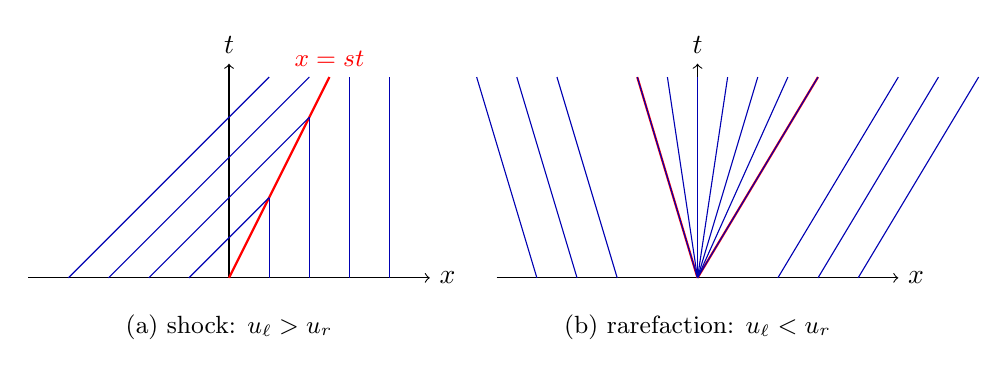
\begin{tikzpicture}[scale=0.85]
  % --- Shock case (left): u_l = 1, u_r = 0, s = 1/2 ---
  \begin{scope}
    \draw[->] (-3,0) -- (3,0) node[right] {$x$};
    \draw[->] (0,0) -- (0,3.2) node[above] {$t$};
    \draw[thick, red] (0,0) -- (1.5,3) node[above] {\small $x=st$};
    % left characteristics: speed u_l = 1, stop on hitting the shock x = t/2
    \foreach \xz in {-2.4,-1.8,-1.2,-0.6}{
      \pgfmathsetmacro{\tm}{min(3,-2*\xz)}
      \draw[blue!70!black] (\xz,0) -- ({\xz+\tm},\tm);
    }
    % right characteristics: speed u_r = 0 (vertical), stop on the shock
    \foreach \xz in {0.6,1.2,1.8,2.4}{
      \pgfmathsetmacro{\tm}{min(3,2*\xz)}
      \draw[blue!70!black] (\xz,0) -- (\xz,\tm);
    }
    \node[below] at (0,-0.4) {\small (a) shock: $u_\ell>u_r$};
  \end{scope}
  % --- Rarefaction case (right) ---
  \begin{scope}[xshift=7cm]
    \draw[->] (-3,0) -- (3,0) node[right] {$x$};
    \draw[->] (0,0) -- (0,3.2) node[above] {$t$};
    \draw[thick, red] (0,0) -- (-0.9,3);
    \draw[thick, red] (0,0) -- (1.8,3);
    \foreach \xz in {-2.4,-1.8,-1.2}{
      \draw[blue!70!black] (\xz,0) -- ({\xz-0.3*3},3);
    }
    \foreach \m in {0,1,...,6}{
      \draw[blue!70!black] (0,0) -- ({-0.9+\m*0.45},3);
    }
    \foreach \xz in {1.2,1.8,2.4}{
      \draw[blue!70!black] (\xz,0) -- ({\xz+0.6*3},3);
    }
    \node[below] at (0,-0.4) {\small (b) rarefaction: $u_\ell<u_r$};
  \end{scope}
\end{tikzpicture}
\caption{Characteristics for the two cases of
Theorem~\ref{thm:riemann-solution}. (a) $u_\ell=1$, $u_r=0$, $s=1/2$:
characteristics on both sides run into the shock $x=st$. (b) Characteristics
fan out from the origin.}
\label{fig:riemann-characteristics}
\end{figure}    % Sections 4--7: weak solutions, non-uniqueness, entropy, Riemann problem

% ---------- Extensions (Section 8) ----------
% Each extension is its own file so it can be cut with a single line.
% =====================================================================
%  Section 8.1--8.3: Cole--Hopf, exact solution, vanishing viscosity.
%  Section 8.4 (Godunov scheme) is in ext_godunov.tex.
% =====================================================================

\section{Extensions}
\label{sec:extensions}

Section~\ref{sec:nonuniqueness} showed that conservation alone leaves infinitely many
weak solutions, and the Oleinik condition restores uniqueness, but it does not
explain \emph{why} nature, or a physical model with a small viscosity, picks that
solution. Can the selected solution be derived from the underlying viscous
equation? This section tests the entropy condition against the two standard selection
mechanisms: vanishing viscosity (Subsections~\ref{subsec:cole-hopf}--%
\ref{subsec:vanishing-viscosity}) and monotone numerical approximation
(Subsection~\ref{subsec:godunov}).

\subsection{The Cole--Hopf transformation}
\label{subsec:cole-hopf}

\begin{theorem}[Cole--Hopf transformation \cite{cole1951,hopf1950}]
\label{thm:cole-hopf}
Let $u\in C^{2,1}(\mathbb{R}\times(0,T))$ solve $u_t+u\,u_x=\nu\,u_{xx}$, with $u$ and
$u_x$ continuous on $\mathbb{R}\times[0,T)$ (so that $c$ below is defined), and set
\begin{equation}
  \label{eq:cole-hopf-def}
  \hat\psi(x,t)=-\frac{1}{2\nu}\int_0^x u(y,t)\,dy,
  \qquad
  c(t)=\int_0^t\Big(\frac{u(0,\tau)^2}{4\nu}-\frac{u_x(0,\tau)}{2}\Big)d\tau,
  \qquad
  \theta(x,t)=\exp\big(\hat\psi(x,t)+c(t)\big)>0 .
\end{equation}
Then $\theta$ solves the heat equation $\theta_t=\nu\,\theta_{xx}$, and
$u=-2\nu\,\theta_x/\theta$.
\end{theorem}

\begin{proof}
Since $c$ depends on $t$ only, $\theta_x/\theta=\hat\psi_x=-u/(2\nu)$, which
gives $u=-2\nu\theta_x/\theta$. For the heat equation, let
$w=\hat\psi_t-\nu\hat\psi_{xx}-\nu\hat\psi_x^2$. Using
$\hat\psi_x=-u/(2\nu)$, $\hat\psi_{xx}=-u_x/(2\nu)$,
$\hat\psi_{xt}=-u_t/(2\nu)$ and $\hat\psi_{xxx}=-u_{xx}/(2\nu)$,
\begin{equation}
  w_x=\hat\psi_{xt}-\nu\hat\psi_{xxx}-2\nu\hat\psi_x\hat\psi_{xx}
  =-\frac{1}{2\nu}\big(u_t+u\,u_x-\nu\,u_{xx}\big)=0 .
\end{equation}
Hence $w$ depends on $t$ only and may be evaluated at $x=0$, where
$\hat\psi(0,t)=0$ gives $\hat\psi_t(0,t)=0$:
\begin{equation}
  w(t)=w(0,t)=\frac{u_x(0,t)}{2}-\frac{u(0,t)^2}{4\nu}=:C(t).
\end{equation}
With $\psi=\hat\psi+c$ we have $c'=-C$, so $\psi_t-\nu\psi_{xx}-\nu\psi_x^2=
C+c'=0$. Since $\theta=e^{\psi}$ satisfies $\theta_t=\theta\psi_t$ and
$\theta_{xx}=\theta(\psi_{xx}+\psi_x^2)$, this is $\theta_t=\nu\theta_{xx}$. (The
factor $e^{c(t)}$ depends on $t$ only, so it affects neither $u=-2\nu\theta_x/\theta$
nor the initial data, as $c(0)=0$; it cannot be omitted, since $e^{\hat\psi}$
satisfies $\partial_t\theta=\nu\theta_{xx}+C(t)\theta$.)
\end{proof}



\subsection{Exact solution via the heat kernel}
\label{subsec:cole-hopf-solution}

By Theorem~\ref{thm:cole-hopf}, a classical solution of \eqref{eq:viscous-burgers}
that is bounded on $\mathbb{R}\times[0,T']$ for each $T'<T$ (this is what makes
$\theta$ obey the growth bound below) corresponds to a solution of the heat
equation with initial data
\begin{equation}
  \label{eq:theta0}
  \theta_0(x) = \exp\left(-\frac{1}{2\nu}\int_0^x u_0(y)\, dy\right)
  \le e^{\|u_0\|_\infty|x|/(2\nu)} .
\end{equation}
The Cauchy problem for the heat equation has a unique solution in the class of
at most $e^{a|x|^2}$ growth \cite[\S2.3.3]{evans2010}, which contains this
data; it is given by
\begin{equation}
  \label{eq:theta-heat-kernel}
  \theta(x,t) = \int_{\mathbb{R}} \frac{1}{\sqrt{4\pi\nu t}}\,
    \exp\left(-\frac{(x-y)^2}{4\nu t}\right) \theta_0(y)\, dy.
\end{equation}
Substituting \eqref{eq:theta0}--\eqref{eq:theta-heat-kernel} into
$u=-2\nu\,\theta_x/\theta$ and differentiating under the integral gives the
\emph{Cole--Hopf formula}
\begin{equation}
  \label{eq:cole-hopf-formula}
  u(x,t) = \frac{\displaystyle\int_{\mathbb{R}} \frac{x-y}{t}\, \exp\left(-\frac{G(x,y,t)}{2\nu}\right) dy}
                {\displaystyle\int_{\mathbb{R}} \exp\left(-\frac{G(x,y,t)}{2\nu}\right) dy},
  \qquad
  G(x,y,t) = \int_0^y u_0(r)\, dr + \frac{(x-y)^2}{2t}.
\end{equation}

\begin{corollary}[Global smoothness; Hopf \cite{hopf1950}]
\label{cor:global-smoothness}
For every bounded measurable $u_0$ and every $\nu>0$, formula
\eqref{eq:cole-hopf-formula} defines a $C^\infty$ solution $u^{(\nu)}$ of
\eqref{eq:viscous-burgers} on $\mathbb{R}\times(0,\infty)$. Moreover
$\|u^{(\nu)}\|_\infty\le\|u_0\|_\infty$, $u^{(\nu)}(\cdot,t)\to u_0$ in
$L^1_{\mathrm{loc}}$ and at every continuity point of $u_0$ as $t\to0^+$, and
$u^{(\nu)}$ is the unique bounded solution with these properties.
\end{corollary}

\noindent For $t>0$, $\theta$ in \eqref{eq:theta-heat-kernel} is smooth and
positive, and for any such solution $\theta$ of the heat equation
$u=-2\nu\theta_x/\theta$ solves \eqref{eq:viscous-burgers}: with
$\psi=\ln\theta$, $\psi_t-\nu\psi_{xx}-\nu\psi_x^2=0$, and differentiating in
$x$ gives $(-u/2\nu)_t-\nu(-u/2\nu)_{xx}-\nu\big((u/2\nu)^2\big)_x=0$, i.e.\
$u_t+u\,u_x=\nu u_{xx}$. This proves the first assertion for merely measurable
$u_0$ (Theorem~\ref{thm:cole-hopf} is not needed in this direction), while the
bound, the sense in which the data are attained, and uniqueness are taken from
Hopf \cite{hopf1950}.

\subsection{The vanishing viscosity limit}
\label{subsec:vanishing-viscosity}

\begin{theorem}[Vanishing viscosity limit \cite{hopf1950}]
\label{thm:vanishing-viscosity}
Let $u_0\in L^\infty(\mathbb{R})$, let $u^{(\nu)}$ be the solution of
\eqref{eq:viscous-burgers} with data $u_0$ given by
\eqref{eq:cole-hopf-formula}, and let $u$ be the entropy solution of
\eqref{eq:inviscid-burgers} with the same data
(Definition~\ref{def:entropy-solution}; for Riemann data,
Theorem~\ref{thm:riemann-solution}). Then $u^{(\nu)} \to u$ pointwise almost
everywhere and in $L^1_{\mathrm{loc}}$ as $\nu \to 0^+$.
\end{theorem}

Hopf's proof \cite{hopf1950} applies Laplace's method to
\eqref{eq:cole-hopf-formula} and shows that $u^{(\nu)}$ converges to the
Lax--Oleinik solution \eqref{eq:lax-oleinik}. Because his work predates Oleinik's
condition, the identification of this limit with $u$ combines the theorem with
Remark~\ref{rem:lax-oleinik} below, which shows that the Lax--Oleinik solution
satisfies \eqref{eq:oleinik}, and with Theorem~\ref{thm:oleinik-uniqueness}. In
short: the viscous solutions converge to the Lax--Oleinik solution (Hopf); that
solution is a weak solution obeying \eqref{eq:oleinik} (Remark~\ref{rem:lax-oleinik});
and weak solutions obeying \eqref{eq:oleinik} are unique, so the limit is $u$.

\begin{remark}[The Lax--Oleinik formula]
\label{rem:lax-oleinik}
As $\nu\to0$ the weight $\exp(-G/2\nu)$ in \eqref{eq:cole-hopf-formula}
concentrates at the minimisers of $y\mapsto G(x,y,t)$. Where the minimiser
$y^*(x,t)$ is unique, the limit is
\begin{equation}
  \label{eq:lax-oleinik}
  u(x,t)=\frac{x-y^*(x,t)}{t},\qquad
  y^*(x,t)=\operatorname*{arg\,min}_y\Big\{V(y)+\frac{(x-y)^2}{2t}\Big\},
  \quad V(y)=\int_0^y u_0 ,
\end{equation}
the \emph{Lax--Oleinik formula} \cite{lax1957,oleinik1957},
\cite[\S3.4.2]{evans2010}; a jump occurs where two minimisers tie. Since
$x\mapsto y^*(x,t)$ is nondecreasing \cite[\S3.4.2]{evans2010}, for $z>0$
\begin{equation*}
  u(x+z,t)-u(x,t)=\frac{z-\big(y^*(x+z,t)-y^*(x,t)\big)}{t}\ \le\ \frac zt,
\end{equation*}
which is \eqref{eq:oleinik}. As \eqref{eq:lax-oleinik} also defines a weak
solution \cite[\S3.4.2]{evans2010}, the Lax--Oleinik solution is an entropy
solution in the sense of Definition~\ref{def:entropy-solution}. The same bound
shows $u(x+,t)-u(x-,t)\le0$ wherever one-sided limits exist: every jump is
downward. The minimiser is unique for almost every $(x,t)$
\cite[\S3.4.2]{evans2010}, so \eqref{eq:lax-oleinik} defines $u$ a.e.
\end{remark}

\begin{remark}[Riemann data and the Lax--Oleinik formula]
\label{rem:riemann-lax-oleinik}
For the data \eqref{eq:general-riemann-data}, $V(y)=u_\ell y$ for $y<0$ and
$V(y)=u_r y$ for $y>0$, so $G(y)=V(y)+(x-y)^2/2t$ has a kink at $y=0$ and
critical points $y_\ell=x-u_\ell t$ (admissible iff $x\le u_\ell t$) and
$y_r=x-u_rt$ (iff $x\ge u_rt$). If $u_\ell<u_r$ and $u_\ell t<x<u_rt$, only the
kink is a minimiser, giving the fan $u=x/t$. If $u_\ell>u_r$ and
$u_rt<x<u_\ell t$, both $y_\ell,y_r$ are admissible, the kink is a local maximum,
and $G(y_\ell)-G(y_r)=(u_\ell-u_r)\big(x-\tfrac{u_\ell+u_r}2t\big)$, so the
minimum switches at $x=\tfrac{u_\ell+u_r}2t$: the Rankine--Hugoniot speed is the
position at which two minimisers tie.\end{remark}

\subsubsection{Viscous shock profiles}
\label{subsubsec:viscous-profiles}

\begin{proposition}[Viscous shock profiles]
\label{prop:viscous-profile}
Let $u_\ell\neq u_r$ and $\nu>0$. Equation \eqref{eq:viscous-burgers} has a
travelling-wave solution $u(x,t)=\phi(x-st)$, with $\phi\in C^2$ bounded,
$\phi(\eta)\to u_\ell$ as $\eta\to-\infty$, $\phi(\eta)\to u_r$ as $\eta\to+\infty$
and $\phi'\to0$ as $\eta\to\pm\infty$, if and only if $u_\ell>u_r$. In that case
$s=(u_\ell+u_r)/2$ and, with $\Delta=u_\ell-u_r$, $\phi$ is unique up to
translation $\eta\mapsto\eta+\eta_0$; the translate with $\phi(0)=s$ is
\begin{equation}
  \label{eq:viscous-profile}
  \phi(\eta)=s-\frac{\Delta}{2}\tanh\!\Big(\frac{\Delta\,\eta}{4\nu}\Big).
\end{equation}
Moreover $\|\phi-(s-\tfrac\Delta2\operatorname{sgn}\eta)\|_{L^1(\mathbb{R})}
=4\ln2\;\nu$, independent of $s$ and $\Delta$.
\end{proposition}

\begin{proof}
Substituting $u=\phi(x-st)$ gives $-s\phi'+\phi\phi'=\nu\phi''$, and
integrating once from $-\infty$ (where $\phi'\to0$),
\begin{equation*}
  \nu\phi'=\tfrac12\phi^2-s\phi-K,\qquad K=\tfrac12u_\ell^2-su_\ell .
\end{equation*}
Letting $\eta\to+\infty$ shows that the right-hand side must also vanish at
$u_r$, so $u_\ell,u_r$ are the two roots of the quadratic: $s=(u_\ell+u_r)/2$
(the Rankine--Hugoniot speed) and
\begin{equation}
  \label{eq:profile-ode}
  \nu\phi'=\tfrac12(\phi-u_\ell)(\phi-u_r).
\end{equation}
By uniqueness for this autonomous ODE, a nonconstant solution cannot cross
either equilibrium $u_\ell,u_r$, so a connecting $\phi$ lies strictly between them. On
$(\min(u_\ell,u_r),\max(u_\ell,u_r))$ the right side of \eqref{eq:profile-ode}
is negative, so $\phi$ is decreasing. If $u_\ell<u_r$ it would have to
increase from $u_\ell$ to $u_r$, a contradiction; if $u_\ell>u_r$,
\eqref{eq:profile-ode} is solved by \eqref{eq:viscous-profile}; any other solution is a translate, by
uniqueness for the ODE. For the $L^1$
distance, by oddness and $\int_0^\infty(1-\tanh\zeta)\,d\zeta=\ln2$,
\begin{equation*}
  \int_{\mathbb{R}}\tfrac\Delta2\Big|\tanh\tfrac{\Delta\eta}{4\nu}-\operatorname{sgn}\eta\Big|\,d\eta
  =\Delta\int_0^\infty\Big(1-\tanh\tfrac{\Delta\eta}{4\nu}\Big)d\eta
  =\Delta\cdot\frac{4\nu}{\Delta}\ln2=4\ln2\,\nu .
\end{equation*}
\end{proof}

Proposition~\ref{prop:viscous-profile} determines which isolated jumps admit a
viscous connecting profile, namely exactly those with $u_\ell>u_r$, of thickness
$O(\nu/\Delta)$; this motivates the Lax condition \eqref{eq:lax-burgers} but does
not by itself select a solution of the initial-value problem. That selection is the
role of Theorem~\ref{thm:vanishing-viscosity}, which together with
Proposition~\ref{prop:entropy-selects-B} excludes $u_A$ of
Section~\ref{sec:nonuniqueness}. As a check, for the shock data $(1,0)$ the
closed-form Cole--Hopf solution (\texttt{cole\_hopf\_riemann.py} \cite{code}) lies at
$L^1(-2,2)$ distance $2.773\,\nu$ from the entropy solution at $t=1$ for
$\nu\le10^{-3}$, matching the layer value $4\ln2\,\nu$ above.     % 8.1--8.3: Cole--Hopf, vanishing viscosity (opens Section 8)
% =====================================================================
%  Section 8.4: Godunov's method.
% =====================================================================

\subsection{Godunov's method}
\label{subsec:godunov}

\subsubsection{The scheme}
\label{subsubsec:godunov-flux}

Let $\mathbb{R}$ be divided into cells $[x_{j-1/2},x_{j+1/2}]$ of width
$\Delta x$, with $t^n=n\Delta t$ and cell averages
$\bar u_j^n=\Delta x^{-1}\int_{x_{j-1/2}}^{x_{j+1/2}}u(x,t^n)\,dx$ approximated by $U_j^n$.
Integrating $u_t+f(u)_x=0$ over a cell and a time step gives
\begin{equation}
  \bar u_j^{n+1} = \bar u_j^n - \frac{\Delta t}{\Delta x}
  \left( F_{j+1/2}^n - F_{j-1/2}^n \right),
  \qquad F_{j+1/2}^n=\frac1{\Delta t}\int_{t^n}^{t^{n+1}}f\big(u(x_{j+1/2},t)\big)\,dt,
\end{equation}
for the exact cell averages $\bar u_j^n$. The scheme replaces $F_{j+1/2}^n$ by a
numerical flux $\widehat f_{j+1/2}$ depending on $U_j^n,U_{j+1}^n$, giving
$U_j^{n+1}=U_j^n-\frac{\Delta t}{\Delta x}(\widehat f_{j+1/2}-\widehat f_{j-1/2})$.
Godunov's method \cite{godunov1959} takes $\widehat f_{j+1/2}$ to be the flux
at $x/t=0$ of the exact Riemann solution with data $(U_j^n,U_{j+1}^n)$
(Theorem~\ref{thm:riemann-solution}):
\begin{equation}
  \label{eq:godunov-flux}
  \widehat f_{j+1/2} = f\big(\omega(0;\, U_j^n, U_{j+1}^n)\big),
\end{equation}
where $\omega(\xi;u_\ell,u_r)$ is the entropy solution with data $(u_\ell,u_r)$ at
$\xi=x/t$. By \eqref{eq:riemann-shock}--\eqref{eq:riemann-rarefaction},
\begin{equation}
  \omega(0; u_\ell,u_r) =
  \begin{cases}
    u_\ell, & u_\ell>u_r,\ \tfrac{u_\ell+u_r}{2}>0, \\
    u_r, & u_\ell>u_r,\ \tfrac{u_\ell+u_r}{2}<0, \\
    u_\ell, & u_\ell\le u_r,\ u_\ell\ge0, \\
    u_r, & u_\ell\le u_r,\ u_r\le0, \\
    0, & u_\ell < 0 < u_r,
  \end{cases}
\end{equation}
the last case corresponding to $\xi=0$ lying inside the fan. If
$u_\ell=-u_r$ the value $\omega(0)$ is ambiguous, but $f(u_\ell)=f(u_r)$, so
\eqref{eq:godunov-flux} is unaffected.

\subsubsection{Stability and convergence}
\label{subsubsec:godunov-convergence}

Monotonicity is the property that makes the scheme entropy-respecting: a scheme is
monotone if raising the data $U_j^n$ never lowers $U_i^{n+1}$, and monotone
conservative schemes cannot create new extrema or oscillations, so they behave like
a viscous regularisation, whereas consistency and conservation alone do not
(Section~\ref{subsubsec:non-entropy}). The scheme is monotone provided the CFL
condition
\begin{equation}
  \label{eq:cfl}
  \Delta t \le \frac{\Delta x}{\max_j |U_j^n|}
\end{equation}
holds, which prevents waves from neighbouring interfaces from reaching
$x_{j+1/2}$ within one step \cite[Ch.~4]{leveque2002}.

\begin{theorem}[{\cite[Theorem~1 and \S1]{crandall1980}}]
\label{thm:godunov-convergence}
Let $u_0\in L^1(\mathbb{R})\cap L^\infty(\mathbb{R})$ with $a\le u_0\le b$ a.e.,
and let $\lambda=\Delta t/\Delta x$ be fixed with
$\lambda\max_{a\le u\le b}|f'(u)|\le1$. Let $u^{\Delta}$ be the piecewise
constant function equal to $U_j^n$ on $[x_{j-1/2},x_{j+1/2})\times[t^n,t^{n+1})$,
where $U_j^0$ is the cell average of $u_0$ and the $U_j^n$ are the Godunov
approximations. Then for every $T>0$
\begin{equation*}
  \lim_{\Delta t\to0}\ \sup_{0\le t\le T}\int_{\mathbb{R}}\big|u^{\Delta}(x,t)-u(x,t)\big|\,dx=0,
\end{equation*}
where $u$ is the Kru\v{z}kov entropy solution \cite{kruzhkov1970} with data $u_0$.
\end{theorem}

The theorem holds for any consistent conservation-form scheme that is monotone on
$[a,b]$ with Lipschitz numerical flux, and Godunov's scheme is such a scheme for
$f''>0$ (\cite[\S1]{crandall1980}); it gives no rate. For Burgers' equation the
Kru\v{z}kov solution is the Oleinik solution of
Theorem~\ref{thm:oleinik-uniqueness}, for the following reason. By
Theorem~\ref{thm:vanishing-viscosity} the Oleinik solution $u$ is the $L^1_{\rm loc}$
limit of viscous solutions $u^{(\nu)}$. These satisfy
$|u^{(\nu)}-k|_t+(\operatorname{sgn}(u^{(\nu)}-k)(f(u^{(\nu)})-f(k)))_x\le\nu|u^{(\nu)}-k|_{xx}$
for every $k\in\mathbb{R}$ (Remark~\ref{rem:entropy-inequality} with $\eta(u)=|u-k|$,
by smooth approximation), and letting $\nu\to0$ gives the same inequality with
$\nu=0$, which is Kru\v{z}kov's definition of an entropy solution. Hence $u$ is a
Kru\v{z}kov solution, and by Kru\v{z}kov's uniqueness theorem \cite{kruzhkov1970} it is the
only one.

\subsubsection{Numerical results}
\label{subsubsec:godunov-results}

Since the Riemann data used below are not in $L^1(\mathbb{R})$, we replace them by $0$
outside $[-5,5]$; as $|u|\le1$ and the numerical domain of dependence over $t\le1$
has half-width $t/\lambda<2.23$, this changes neither the exact nor the computed
solution on $[-2,2]\times[0,1]$. Since $\max_j|U_j^n|=1$ in the experiments,
$\Delta t=0.45\,\Delta x/\max_j|U_j^n|$ gives the constant $\lambda=0.45$ of the
theorem (the final step, shortened to end at $t=1$, has smaller $\lambda$).
The scheme was implemented in \texttt{godunov.py} \cite{code} on $x\in[-2,2]$ with $N$
cells, cell-averaged initial data and outflow boundary conditions. The rarefaction data $(0,1)$ and shock data $(1,0)$ were run to $t=1$, with
error $\sum_j\int_{I_j}|U_j-u_{\rm exact}(x,1)|\,dx$ against the solution of
Theorem~\ref{thm:riemann-solution} (not cell-averaged, so a cell containing the
shock is scored against the discontinuity itself). The code checks that the
case-based flux \eqref{eq:godunov-flux} agrees with the closed form on random state
pairs, that mass is conserved up to boundary flux, and that enlarging the domain to
$[-4,4]$ changes the values on $[-2,2]$ by at most $3\times10^{-14}$.
Figure~\ref{fig:godunov-results} shows $N=400$: the computed shock lies at
$x=st=0.5$ and the fan has slope $1/t$, with no oscillation.

\begin{figure}[htbp]
\centering
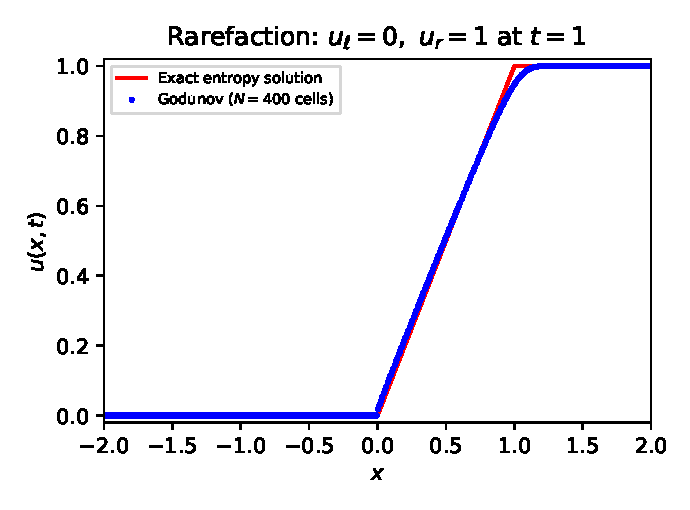
\includegraphics[width=0.44\textwidth]{figures/godunov_rarefaction.pdf}
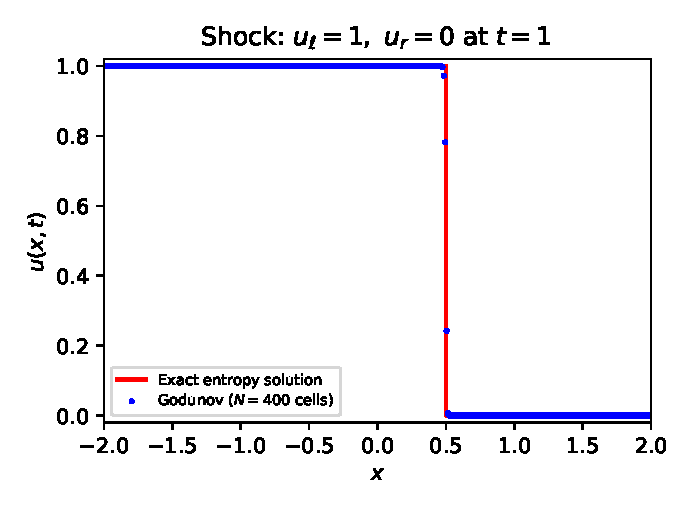
\includegraphics[width=0.44\textwidth]{figures/godunov_shock.pdf}
\caption{Godunov scheme (dots, $N=400$) against the exact entropy solution
(solid) at $t=1$. Left: rarefaction data $(0,1)$. Right: shock data
$(1,0)$. Code: \cite{code}.}
\label{fig:godunov-results}
\end{figure}

\begin{table}[htbp]
\centering
\begin{tabular}{r r r r r r}
  $N$ & $\Delta x$ & $L^1$ (rarefaction) & order & $L^1$ (shock) & order \\\hline
  200  & $2.0\times10^{-2}$ & $3.05\times10^{-2}$ & --- & $9.91\times10^{-3}$ & --- \\
  400  & $1.0\times10^{-2}$ & $1.82\times10^{-2}$ & 0.74 & $4.98\times10^{-3}$ & 0.99 \\
  800  & $5.0\times10^{-3}$ & $1.07\times10^{-2}$ & 0.77 & $2.50\times10^{-3}$ & 0.99 \\
  1600 & $2.5\times10^{-3}$ & $6.14\times10^{-3}$ & 0.80 & $1.24\times10^{-3}$ & 1.01 \\
  3200 & $1.25\times10^{-3}$ & $3.48\times10^{-3}$ & 0.82 & $6.23\times10^{-4}$ & 0.99 \\
  6400 & $6.25\times10^{-4}$ & $1.95\times10^{-3}$ & 0.84 & $3.13\times10^{-4}$ & 0.99
\end{tabular}
\caption{$L^1$ errors at $t=1$ and observed orders $\log_2(e_{N/2}/e_N)$.
All $N$ are multiples of $8$, so the shock lies on a cell interface. Code: \cite{code}.}
\label{tab:godunov-conv}
\end{table}

\paragraph{Shock.} Here $E/\Delta x$ is the shock error measured in cell widths, so a value $c$ means the
computed profile differs from the sharp shock by an amount equal to $c$ cells'
worth of mass. The shock $x=st=0.5$ lies on a cell interface iff $8\mid N$, which
matters because otherwise the cell containing it holds a mixed initial average and
the initial error depends on where the discontinuity falls inside that cell;
for such $N$ the ratio $E/\Delta x$ lies between $0.495$ and $0.501$ and the
observed order is $\approx1$ (Table~\ref{tab:godunov-conv}). On misaligned grids
($N=97,\dots,103$) it ranges from $0.55\,\Delta x$ to $0.66\,\Delta x$, so orders
computed between misaligned and aligned resolutions are unreliable (from $N=100$ to
$200$ one would obtain $1.40$); this is why the table uses $N=200\cdot2^k$.

\paragraph{Rarefaction.} The observed orders $0.74,0.77,0.80,0.82,0.84$ are still
increasing, so these experiments do not establish a first-order rate. In fact
$E/\Delta x$ grows by $0.30$ to $0.34$ per halving of $\Delta x$, roughly linearly in
$\ln(1/\Delta x)$, which is consistent with, but does not prove, an error of the form
$\Delta x\,(c+c'\ln(1/\Delta x))$, that is, first order up to a logarithm. The error is
concentrated near the fan but not at its corners: the fan interior $0.2<x<0.8$
carries about a third of it, so the rate has not stabilised.

\subsubsection{Numerical diffusion as vanishing viscosity}
\label{subsubsec:numerical-viscosity}

For the shock data the scheme is monotone, so by the discrete maximum principle
all states remain in $[0,1]$. All characteristic speeds are then nonnegative, so
the Godunov flux is the upwind flux $f(U_j^n)$, and the scheme reads
$U_j^{n+1}=U_j^n-\lambda(f(U_j^n)-f(U_{j-1}^n))$, $\lambda=\Delta t/\Delta x$.
The mechanism is that upwinding averages information from one side, and the leading
error of such an average is a diffusion term. Taylor expansion gives the modified equation
\begin{equation}
  \label{eq:modified-equation}
  u_t+u\,u_x=\frac{\Delta x}{2}\big(u(1-\lambda u)\,u_x\big)_x+O(\Delta x^2),
\end{equation}
a Burgers-type equation in conservative form, with state-dependent viscosity
$\nu(u)=\tfrac{\Delta x}2u(1-\lambda u)$, nonnegative exactly under
\eqref{eq:cfl}. In the scaled variable $\eta=(x-t/2)/\Delta x$, its travelling shock $1\to0$ of
speed $\tfrac12$ satisfies $\tfrac12u(1-\lambda u)u_\eta=\tfrac12u(u-1)$, that is,
\begin{equation}
  \frac{du}{d\eta}=\frac{u-1}{1-\lambda u},\qquad
  \eta(u)=\eta_0+(1-\lambda)\ln(1-u)-\lambda u .
\end{equation}
The profile decays exponentially to $1$ as $\eta\to-\infty$ and reaches $0$ at
a finite $\eta_0$, which conservation of mass fixes as $\eta_0=1-\lambda/2$. The
$L^1$ distance from the sharp shock is then
\begin{equation}
  \frac{\|u-u_{\rm exact}\|_{L^1}}{\Delta x}
  =2\int_0^{u_0}\frac{u(1-\lambda u)}{1-u}\,du,\qquad
  (1-\lambda)\ln(1-u_0)-\lambda u_0=-\Big(1-\frac\lambda2\Big).
\end{equation}
Table~\ref{tab:numerical-viscosity} compares this with the measured shock error on
aligned grids, where $\lambda$ equals the CFL number since $\max|U|=1$
(\texttt{numerical\_viscosity.py} \cite{code}).

\begin{table}[htbp]
\centering
\begin{tabular}{c c c c}
  CFL $=\lambda$ & measured ($N=1600$) & predicted & (pred.$-$meas.)/meas. \\\hline
  0.10 & 0.626 & 0.686 & $+9.4\%$ \\
  0.45 & 0.496 & 0.511 & $+3.1\%$ \\
  0.80 & 0.352 & 0.342 & $-3.0\%$ \\
  0.95 & 0.300 & 0.272 & $-9.3\%$
\end{tabular}
\caption{Shock $L^1$ error divided by $\Delta x$: measured (grids with $8\mid N$)
against the modified-equation prediction (code: \cite{code}).}
\label{tab:numerical-viscosity}
\end{table}

The prediction is within $10\%$ throughout (the CFL $0.95$ value is not yet
asymptotic: $0.334$ at $N=400$). Equating the error with $4\ln2\,\nu_{\rm eff}$
(Proposition~\ref{prop:viscous-profile}, $s=\tfrac12$, $\Delta=1$) defines an
effective viscosity: the measured $0.50\,\Delta x$ gives
$\nu_{\rm eff}\approx0.179\,\Delta x$ and the modified-equation profile gives
$0.184\,\Delta x$, so the effective viscosity vanishes with the mesh, the numerical
analogue of the mechanism behind Theorem~\ref{thm:vanishing-viscosity}. That theorem
concerns constant physical viscosity and does not itself give convergence of the
scheme, whose modified equation is degenerate; convergence is the content of
Theorem~\ref{thm:godunov-convergence}. The agreement of constants is empirical
evidence for the modified equation, not a proof: since
\eqref{eq:modified-equation} presupposes controlled derivatives that grow under
refinement inside a layer of width $O(\Delta x)$, the expansion is formal there, and
the sign change of the discrepancy across CFL numbers shows the agreement is only
approximate.

\subsubsection{A consistent scheme that selects the wrong solution}
\label{subsubsec:non-entropy}

Consider the flux $\widehat f_{j+1/2}=f(U_j)$ if $\tfrac12(U_j+U_{j+1})>0$ and
$f(U_{j+1})$ otherwise, which is consistent and conservative but not monotone.
For the Riemann data $U_j=-1$ ($j\le0$), $U_j=+1$ ($j>0$) every numerical flux
equals $f(\pm1)=\tfrac12$, so $U^{n+1}=U^n$ exactly and the scheme returns the
stationary upward jump, the analogue for these data of $u_A$ in
Section~\ref{sec:nonuniqueness} (a weak solution by
\eqref{eq:rankine-hugoniot-burgers} with speed $0$, but not an entropy solution).
Godunov's flux at the same interface is $f(0)=0$, and the resulting scheme
produces instead the fan $u=x/t$ of Theorem~\ref{thm:riemann-solution}. At $t=1$ the $L^1(-2,2)$
distance to the entropy solution is $1.000$ for the non-monotone scheme for all
$N=200,400,800$, since $\int|\operatorname{sgn}x-\operatorname{clip}(x,-1,1)|\,dx=1$, while for
Godunov's scheme it is $6.1\times10^{-2}$, $3.6\times10^{-2}$,
$2.1\times10^{-2}$. By the Lax--Wendroff theorem \cite[Ch.~12]{leveque2002}, if the approximations
of a consistent conservative scheme remain bounded and converge a.e.\ (or in
$L^1_{\rm loc}$), the limit is a weak solution, so consistency and conservation
alone do not select the entropy solution. Monotonicity
(Theorem~\ref{thm:godunov-convergence}) is a sufficient condition for convergence
to it, though not a necessary one for every scheme.    % 8.4: Godunov's method

\section{Conclusion}
\label{sec:conclusion}

The weak formulation fixes the speed of a shock through the Rankine--Hugoniot
condition, but it does not fix which discontinuities are admissible: already for
Riemann data there are infinitely many weak solutions
(Section~\ref{sec:nonuniqueness}). The Oleinik condition, whose local form at a
jump is the Lax condition $u_\ell>u_r$, selects exactly one of them
(Sections~\ref{sec:entropy-condition}--\ref{sec:riemann-problem}). This is the
solution selected by the viscous Burgers regularisation: the Cole--Hopf solutions
converge to it (Theorem~\ref{thm:vanishing-viscosity},
Remark~\ref{rem:lax-oleinik}), and a viscous travelling wave connecting $u_\ell$
to $u_r$ exists if and only if $u_\ell>u_r$
(Proposition~\ref{prop:viscous-profile}).

Godunov's scheme selects the same solution. Its shock error is $0.50\,\Delta x$
on aligned grids, and the modified equation \eqref{eq:modified-equation} gives an
effective viscosity of roughly $0.18\,\Delta x$ that vanishes with the mesh (a
heuristic consistency check, since the expansion is formal in the shock layer), while a
consistent conservative but non-monotone flux converges to the non-entropy weak
solution (Section~\ref{subsubsec:non-entropy}). The numerics are consistent with
Theorem~\ref{thm:godunov-convergence} \cite{crandall1980}, which supplies the
convergence statement. Taken together, the results show that conservation
determines the speed of a shock, while entropy, whether imposed through the
Oleinik condition, through vanishing viscosity, or through a monotone numerical
scheme, determines which shocks occur.

Several questions remain outside the scope of this paper. We restricted to
bounded data and to the strictly convex flux $u^2/2$, where the Oleinik bound and
the Lax condition are available; for general fluxes, systems and several space
dimensions one must work with Kru\v{z}kov's entropy inequalities or Oleinik's
condition~E, and uniqueness and convergence are then much harder. The rarefaction
experiments did not settle the asymptotic rate of Godunov's scheme, and the
agreement of the effective viscosity with the modified-equation prediction is
empirical only. The picture established here for Burgers' equation, that
discontinuities are admissible exactly when they are limits of viscous layers, is
the model for the entropy conditions of more general conservation laws.

\bibliographystyle{plain}
\bibliography{references}

\end{document}